
\section{Introduction}
\label{sec:review:introduction}
CONFIRMATION REPORT
Several short treatises follow the introduction: on cardiac anatomy; on electrophysiology; on methods in electrophysiological modelling; ending with some theory on imaging, registration and segmentation.
CONFIRMATION REPORT

\begin{figure*}[thbp]
\centerline{
\begin{tabular}{cc}
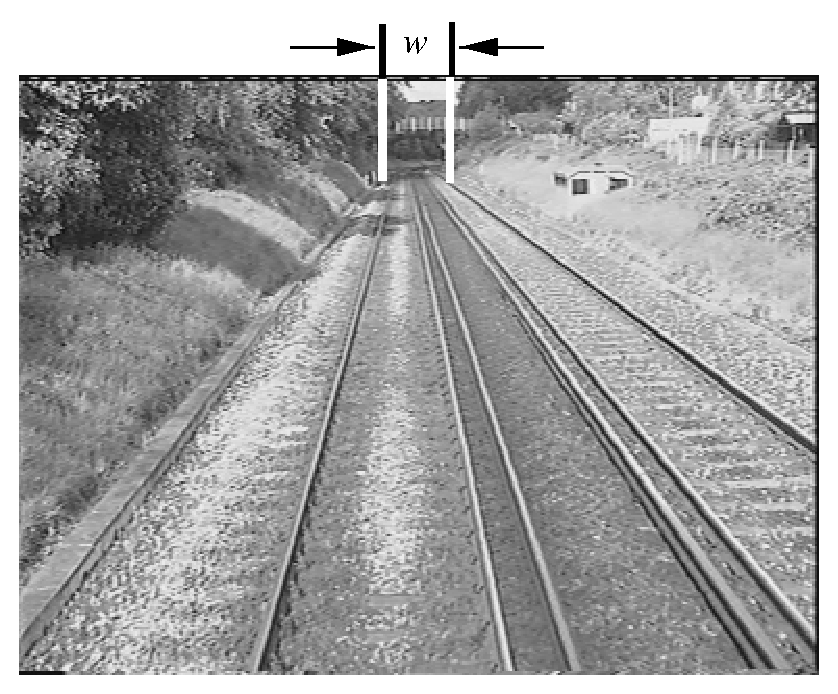
\includegraphics[width=65mm]{\localpath/Figs/calibim} &
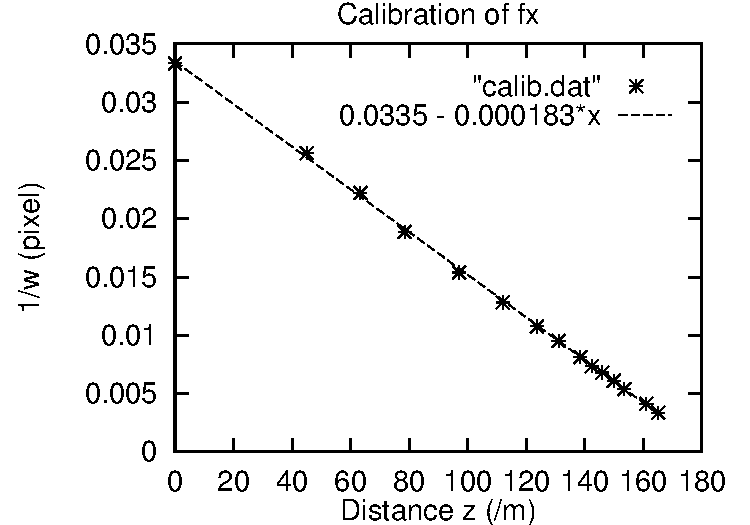
\includegraphics[width=85mm]{\localpath/Figs/calib} \\
(a) & (b)
\end{tabular}
}
\caption{\label{fig:review:calib}
(a) Image and 
(b) measured value of $1/w$ against $z$, and the fitted
straight line.
The slope 
is $1/f_xW = 1.83 \times 10^{-4}$pix$^{-1}$.m$^{-1}$
and the $z$-intercept is $D_o=183$m.
}
\hrule
\end{figure*}


\begin{equation}
\label{eq:review:rubbish}
a = \int_{0}^{1} x^{47} dx ~,
\end{equation}

\section{Algorithms in boxes}
The concensus is that it is best to put algorithms in boxes in
figures, as illustrated in Figure~\ref{fig:review:alg1}.

\begin{figure}
\centerline{\fbox{
\begin{minipage}{75mm}
\begin{algorithmic}
\REQUIRE $n \geq 0$
\ENSURE $y = x^n$
\STATE $y \Leftarrow 1$
\STATE $X \Leftarrow x$
\STATE $N \Leftarrow n$
\WHILE{$N \neq 0$}
\IF{$N$ is even}
\STATE $X \Leftarrow X \times X$
\STATE $N \Leftarrow N / 2$
\ELSE[$N$ is odd]
\STATE $y \Leftarrow y \times X$
\STATE $N \Leftarrow N - 1$
\ENDIF
\ENDWHILE
\end{algorithmic}
\end{minipage}
}}
\caption{\label{fig:review:alg1}
An algorithm in a box for finding the value of a number taken to a
non-negative power.}
\hrule
\end{figure}

\section{Cardiac Anatomy}
TRANSFER THESIS
  The heart is a pump which circulates blood through the lungs and around the body. Throughout a human life, the heart contracts approximately 100,000 times per day, beating around 2.5 billion times in an average 66-year lifetime. The heart is divided into four chambers, two superior atria and two inferior ventricles. Deoxygenated blood from the body flows into the right atrium and into the right ventricle, from where it is pumped through the lungs in order to exchange CO$_2$ with oxygen. Blood returns from the lungs and enters the left atrium and subsequently the left ventricle. Finally, the left ventricle pumps blood back out to the body via the aorta, the widest artery in the body. Retrograde flow through the aorta back into the left ventricle is prevented by the aortic valve.
  
  \begin{figure}[htbp]
    \centering
    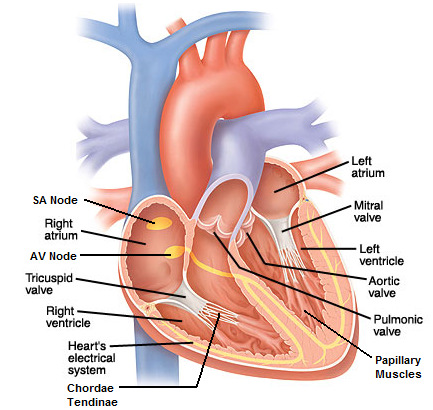
\includegraphics[width=0.6\textwidth]{Ch2/Figs/interior_heart_anatomy}
    \caption{Schematic of the main anatomical features and structures of the heart. Blue vessels carry deoxygenated blood and red vessels oxygenated blood. Note the thicker walls of the left ventricle, to provide enough pressure to force blood around the entire body. The two atrioventricular valves, the tricuspid and the mitral valves, are labelled. From the Ed Dardanell Heart and Vascular Centre (www.forbesheartcenter.com).}
    \label{fig:heart}
  \end{figure}  

The heart walls are comprised mostly of striated muscular tissue known as myocardium. The outer, middle and inner heart walls are termed the epicardium, mid-myocardium and endocardium, respectively. At the cellular level, myocytes are the long oblate myocardial cells, locally aligned with each other. Myocytes are further arranged into discrete myocardial sheets, separated by cleavage planes, as seen in Figure~\ref{fig:sheets}. The myocytes in each sheet will contract in a unified direction and the sheets will slide over each other, maximising the volume output and mechanical efficiency of the heart. A muscular septal wall through the centre of the heart separates oxygenated blood in the right chambers from deoxygenated blood in the left. The eponymous atrioventricular valves prevent blood from leaking back into the atria from the ventricles; these are controlled by the papillary muscles, contractile pillars connected to the valves at their tip and to the endocardium at their base.

  \begin{figure}[htbp]
    \centering
    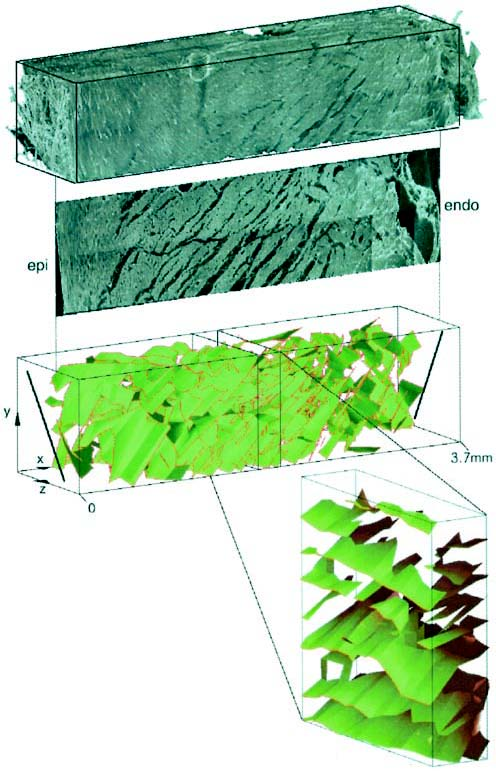
\includegraphics[width=0.6\textwidth]{Ch2/Figs/sheets}
    \caption{The top cuboid is a small volume of rat left ventricular myocardium from \cite{Hooks:2002p442}, reconstructed from a series of 2-D multiple histological images. Just below, a transmural slice from the reconstructed volume shows a complex network of cleavage planes that course between layers of myocytes. Each layer is of around 80$\mu$m thick. The extracted cleavage planes are shown below in green, through the entire rat tissue block and a smaller midwall subsection. Myofiber orientation is shown on the epicardial and endocardial surfaces.}
    \label{fig:sheets}
  \end{figure}

  The vascular system is divided at the heart into two subsystems: the pulmonary vascular system, which transports blood from the right ventricle, through the lungs, and back to the left atrium; and the systemic vascular system, which carries blood from the left ventricle, around the rest of the body, and back to the right atrium. Part of the systemic system is the coronary vascular system, supplying the heart tissue with oxygen and nutrients and removing waste. The main arteries supplying the myocardium stem from the root of the aorta, immediately above the aortic valve, and run along the outer surface of the heart; they are thus named the epicardial coronary arteries. The positioning of the coronary arteries on the surface, away from the high systolic pressures of the endocardium, allow them to remain turgid and autoregulate to supply the heart tissue with appropriate blood flow.
TRANSFER THESIS


\section{Cardiac Electrophysiology}
\label{sec:electrophysiology}
  \subsection{Myocyte Excitation}
  \label{sub:myocyte_excitation}
    Cardiomyocytes contract as a result of an external electrical stimulus. When at rest, a myocyte has a negative membrane potential, around -90mV. Stimulation above a certain threshold causes depolarisation across the cell membrane, as voltage-gated ion channels are activated and positive ions flood into the cell. The controlled influx and efflux of ions such as Na$^+$, K$^+$, Ca$^{2+}$ and Cl$^-$ through various gates, pumps and exchangers eventually ensures the repolarisation of the cell. The form of the transmembrane potential spanning one complete depolarisation/repolarisation cycle is known as an action potential. Gap junctions between adjacent cells ensure a fast and robust propagation mechanism by boulstering this electrical coupling.
  
  \subsection{Activation Sequence}
  \label{sub:activation_sequence}
    Contraction of the heart is controlled by a complex sequence of electrical activation. The sino-atrial node or pacemaker, positioned at the top of the right atrium (see Figure~\ref{fig:heart}), is a cluster of self-excitable myocytes that depolarises at a regular interval, dictating the rate of heart pumping. From there a depolarising wave quickly spreads across the right and left atria, so that they contract in unison and force blood into the ventricles. An electrical barrier isolates the atria from the rest of the heart, and the atrioventricular node provides the only pathway to the ventricles. It delays the signal to allow the atria to contract fully, before stimulating the Purkinje fibres via the bundle of His. The Purkinje fibres are long transduction cells sheathed in an insulating layer of fat, much like neurons. They comprise a network that runs from the bundle of His along the endocardium and through the ventricular cavities, dividing dentritically across both ventricles to carry the electrical signal throughout the ventricular walls. From here, the action potential spreads through the myocardium from endo-~to epicardium, effecting a synchronised contraction of the ventricles and pumping blood to the lungs and body.
    
    Pathological deviations from this highly coordinated electromechanical process severely debilitate cardiac output. Arrhythmia occurs when a reentrant spiral wave manifests within the myocardium, overriding the natural contraction sequence controlled by the sino-atrial node. At the centre of the reentrant wave is a phase singularity, a small area of ambiguous activation that acts as the organising node of the arrythmia. These more organised arrhythmias can degenerate further into more complex arrhythmic episodes termed fibrillation, as the reentrant wave breaks up into smaller, more chaotic fragments. Cardiac output during fibrillation is close to zero as asynchronous fluttering ensues, and the condition is fatal within a few minutes. By far the most common treatment at this stage is defibrillation therapy, where high voltages are applied across the heart via metal plates placed either side of the chest cavity.

\section{Electrophysiological Modelling}
\label{sec:electrophysiological_modelling}
  In creating realistic and powerful cardiac models, it is necessary to represent faithfully the electrophysiological processes of the heart at both the cellular and the tissue level. The bidomain model attempts to unify these two scales, by representing the extra-~and intracellular spaces in cardiac tissue as two continua, such that two electrical potential fields $\phi_\text{e}$ and $\phi_\text{i}$ are defined across the tissue space. The transmembrane potential difference is then given by
  
  \begin{equation}
    v = \phi_\text{i} - \phi_\text{e}.
  \end{equation}
  
  The bidomain equations are a pair of coupled differential equations that are based on a reaction-diffusion model of ion flux. They result from imposing conservation of ions and charge throughout the domain. They can be expressed as
  
  \begin{align}
    \beta \left( C_\text{m}\frac{\partial v}{\partial t} + I_\text{ion}\left( \boldsymbol\eta, v \right) \right) - \nabla \cdot \left( \sigma_\text{i} \nabla \phi_\text{i} \right) &= I_\text{istim}, \\
      \nabla \cdot \left( \sigma_\text{e} \nabla \phi_\text{e} +  \sigma_\text{i} \nabla \phi_\text{i} \right) &= I_\text{estim},
  \end{align} 
  
  where $\beta$ is the membrane surface to volume ratio, $C_\text{m}$ is the specific membrane capacitance, $\sigma_\text{e}$ and $\sigma_\text{i}$ are the extra- and intracellular conductivity tensors, and $I_\text{estim}$ and $I_\text{istim}$ are currents into the two domains due to external stimulus. Cardiac tissue exhibits anisotropic conductivity, transmitting current much more readily along the tubular muscle fibres than across them. Accordingly, the principal eigenvectors of $\sigma_\text{e}$ and $\sigma_\text{i}$ are closely aligned with the local myocardial fibre direction. $I_\text{ion}$ is the ionic current from the extracellular into the intracellular domain. In the simplest passive implementation of the bidomain equations, it would be a term linear in $v$, with the proportionality constant equivalent to the conductance per unit area of the cell membrane. This, however, is highly unrealistic and in practice, $I_\text{ion}$ is a complex function, associated with a non-linear cell electrophysiology model. In this case, $\boldsymbol\eta$ is a vector of the state variables that parameterise the cell model. The cell model dynamics are governed by the set of equations
  
  \begin{equation}
    \frac{\partial \boldsymbol\eta}{\partial t} = \mathbf{f}\left(\boldsymbol\eta, v \right).
  \end{equation}
  
  The monodomain model is a simplification of the bidomain model, based on the assumption that the intra- and extracellular conductivity tensors are linearly dependent i.e. they only differ by a constant scalar factor. The two potentials $\phi_\text{e}$ and $\phi_\text{i}$ are amalgamated, so that only the potential difference $v$ is parameterised. Whilst less accurate, the resulting set of equations often require orders of magnitude less computation. Yet this advantage cannot be exploited for all purposes, since the regime cannot handle conductivity through baths, interstitial spaces and anywhere in the absence of tissue.
  
  The efficient and rigorous solution of these equations over a realistic 3-D geometry is a highly complex task, and remains the ongoing effort of many teams of experts in the field. Detailed knowledge of several fields is necessary, including numerics, algorithms, parallel computing and software design practices. In this thesis, we leverage two advanced cardiac simulation packages for these purposes, Cardiac Arrhythmias Research Package (CARP) and Cancer, Heart And Soft Tissue Environment (CHASTE).

\section{Segmentation}
\subsection{Imaging (From transfer, needs to be split into Seg and Reg)}
\label{imaging}
Medical images from a variety of modalities can be used to develop computational meshes that accurately represent cardiac geometry and structure. It is a common problem in medical imaging to match one image to another for the purposes of comparison and validation, or to combine the information gleaned from both. This process is called registration. Physical regions, objects and features must also be identified from raw image data, for example, a section of the brain or the vessels in the heart. The automation of this identification is known as segmentation. The Insight Toolkit \cite{Yoo:2002p160}, or ITK, is an open-source software toolkit written in C++, used primarily for performing registration and segmentation. It provides a high-level registration framework into which a large selection of functional modules can be swapped, enabling the developer to tailor the registration pipeline to the requirements of the data. The framework consists of the two images to be coregistered, and four main components: a transform, an interpolator, a fitness metric and an optimiser.

If we think of an image as a function of an n-dimensional point in space, one of the images is designated as fixed, while the other is marked as moving. The transform maps grid points in the fixed image to the equivalent point in the moving image. In general, the mapped points will not fall exactly on grid points in the moving image, and so the interpolator generates a value based on the nearby grid points. For example, it might just use the value of the closest grid point, or it might linearly interpolate the nearest neighbours. Once this is completed, the metric compares the fixed image to the resampled moving image and provides a measure of their similarity, along with other information including the gradient of the similarity measure in the parameter space of the transform. Finally, the optimiser uses the information provided by the metric to decide upon a new transform, in an attempt to generate a better similarity value and thus marry the two images more closely. This iterative process is repeated until a minimum threshold for improvement is reached and final parameters are settled on. Figure~\ref{fig:framework} gives a diagrammatic overview of the relationship between the components of the registration framework.

\begin{figure}[htbp]
  \centering
  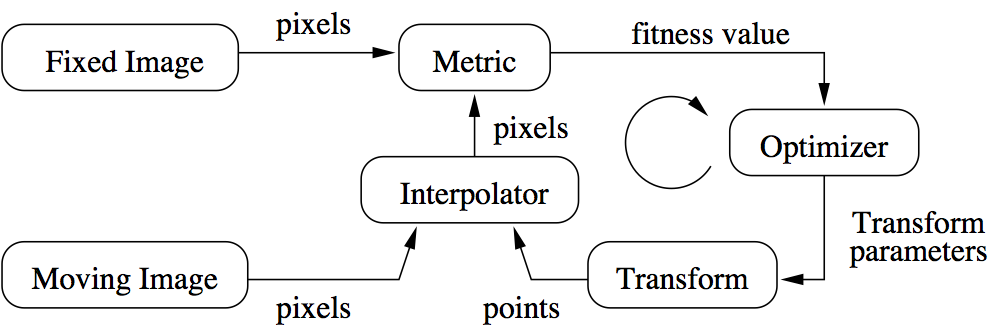
\includegraphics[width=0.85\textwidth]{Ch2/Figs/framework}
  \caption{A schematic of the ITK registration framework. An initial transform is applied to the grid points of the fixed image and an interpolator provides values for each pixel, based on the moving image. The original fixed image and the resampled moving image are then compared by the metric, almost always in a pixelwise fashion, to provide a single-valued measure of fit, and a gradient of this measure with respect to each parameter defining the transform. The optimiser then chooses new transform parameters in an effort to improve the fitness value. The process iterates to convergence.}
  \label{fig:framework}
\end{figure}

\section{Registration}
